%%%%%%%% ICML 2019 EXAMPLE LATEX SUBMISSION FILE %%%%%%%%%%%%%%%%%

\documentclass{article}

% Recommended, but optional, packages for figures and better typesetting:
\usepackage{microtype}
\usepackage{graphicx}
\usepackage{subfigure}
\usepackage{booktabs} % for professional tables

% hyperref makes hyperlinks in the resulting PDF.
% If your build breaks (sometimes temporarily if a hyperlink spans a page)
% please comment out the following usepackage line and replace
% \usepackage{icml2019} with \usepackage[nohyperref]{icml2019} above.
\usepackage{hyperref}

% Attempt to make hyperref and algorithmic work together better:
\newcommand{\theHalgorithm}{\arabic{algorithm}}

% Use the following line for the initial blind version submitted for review:
\usepackage[accepted]{icml2019}

% If accepted, instead use the following line for the camera-ready submission:
%\usepackage[accepted]{icml2019}

% The \icmltitle you define below is probably too long as a header.
% Therefore, a short form for the running title is supplied here:
\icmltitlerunning{Fine grained action recognition in sports videos}

\begin{document}

\twocolumn[
\icmltitle{Fine grained action recognition in sports videos}

% It is OKAY to include author information, even for blind
% submissions: the style file will automatically remove it for you
% unless you've provided the [accepted] option to the icml2019
% package.

% List of affiliations: The first argument should be a (short)
% identifier you will use later to specify author affiliations
% Academic affiliations should list Department, University, City, Region, Country
% Industry affiliations should list Company, City, Region, Country

% You can specify symbols, otherwise they are numbered in order.
% Ideally, you should not use this facility. Affiliations will be numbered
% in order of appearance and this is the preferred way.

\begin{icmlauthorlist}
\icmlauthor{Amit Nagpal (anagpal1@stanford.edu)}{}
\end{icmlauthorlist}

% You may provide any keywords that you
% find helpful for describing your paper; these are used to populate
% the "keywords" metadata in the PDF but will not be shown in the document
\icmlkeywords{Machine Learning, ICML}

\vskip 0.2in
]

% this must go after the closing bracket ] following \twocolumn[ ...

% This command actually creates the footnote in the first column
% listing the affiliations and the copyright notice.
% The command takes one argument, which is text to display at the start of the footnote.
% The \icmlEqualContribution command is standard text for equal contribution.
% Remove it (just {}) if you do not need this facility.

%\printAffiliationsAndNotice{}  % leave blank if no need to mention equal contribution
%\printAffiliationsAndNotice{\icmlEqualContribution} % otherwise use the standard text.

\begin{abstract}
Video, today, is searched and browsed primarily by its cover. To make “Stephen Curry’s 3-pointers” accessible, publishers must create a separate video just for Stephen Curry’s 3-pointers and label it as such. This is inefficient and has not scaled for obvious reasons. Moreover, an increasing population of sports fans do not wish to consume the entirety of every game. They are only interested in watching key games and “interesting parts” of all other games. Finer grained consumption of video content, through finer grained tagging such as action recognition, is key to the ecosystem of sports.

Unlike in everyday life, action recognition in sports is particularly hard due to the chaotic nature of game play. Occlusion is everywhere, players take on extreme body postures and subtle variations mean completely different moves. It is tough to scale, due to the expense of generating training data for each possible move and its variations. Our motivation for this project is to break down moves and learn to classify their common pool of semantic components such as run, jump and dribble in a multiplayer sports setting. We then apply the learning to identify domain specific fine grained moves. For this project we focus on moves in NBA.
\end{abstract}

\section{Introduction}
\label{introduction}
Action recognition in sports is an important area of research in Computer Vision. It has implications beyond consumption by sports fans. Once indexed it can be used by coaches, allowing them to pull from the vast repository of search-able fine grained moves, that they can then analyze and train on. It can be used by students to self learn from an endless stream of sports videos posted on the web. It can be used for automatic highlight generation for less known and hard to access games not hosted by NBA, NFL for example. Once available for any sports video ever recorded, action instances can be used as a basis for entity / athlete "similar to" recommendations, providing a rich platform for the discovery of new stars in the sports. Applications are endless.

Equally importantly it provides us with the motivation of pushing the state of the art in one of the most complex settings in computer vision. Team sports such as NBA involve a large number of players moving rapidly, often unpredictably and frequently converging into a very small area "over the top of each other", with hundreds of audiences in the background. This magnifies the challenges of occlusion, player identification, pose detection, tracking and other classic problems studied in computer vision. 

\begin{figure}[ht]
\vskip 0.15in
\begin{center}
\centerline{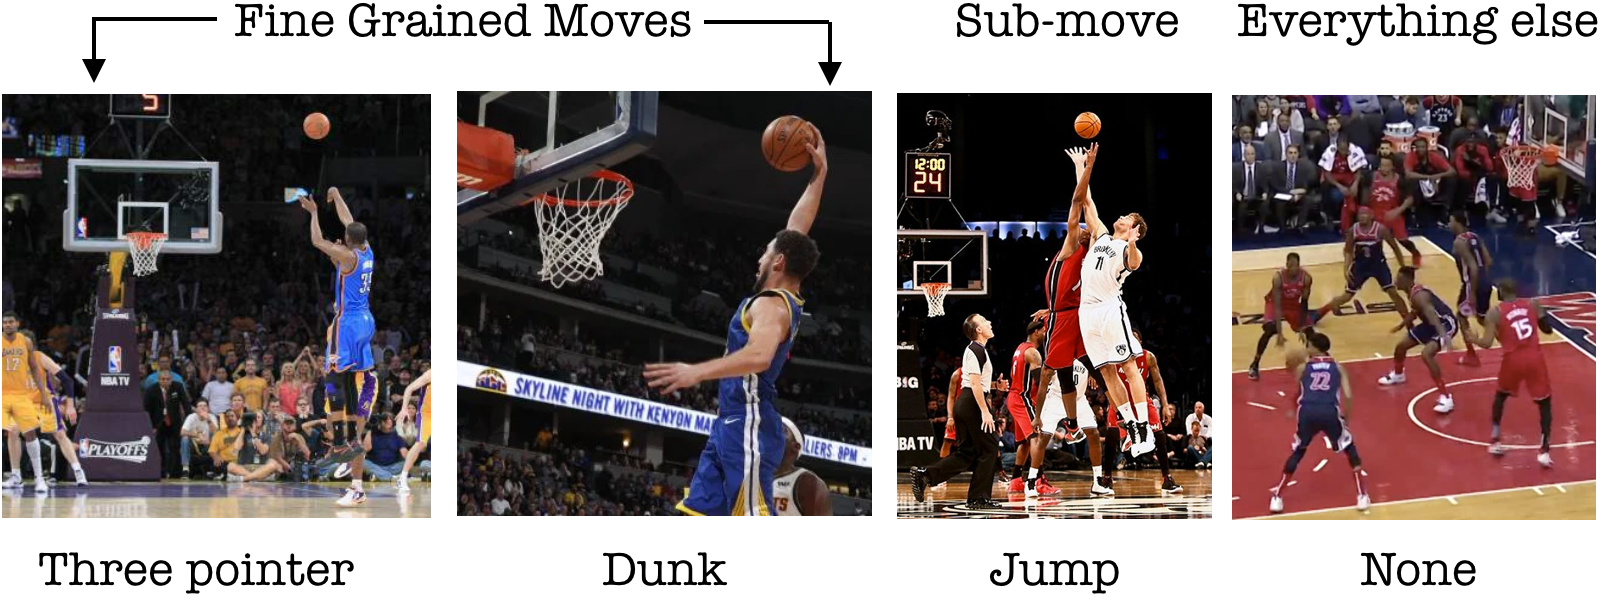
\includegraphics[width=\columnwidth]{Classes.png}}
\caption{Classes}
\label{fig:classes}
\end{center}
\vskip -0.2in
\end{figure}

In this paper we explore the task of building models that can classify a video segment to contain low level semantic sub-moves (jump, dribble etc) as well as fine grained sports specific moves (three pointer, dunks, ..). We limit the scope of this project to classes shown in Figure~\ref{fig:classes}. Our prediction inputs and model experiments are shown in Figure~\ref{fig:e2e}:

\begin{figure}[ht]
\vskip 0.15in
\begin{center}
\centerline{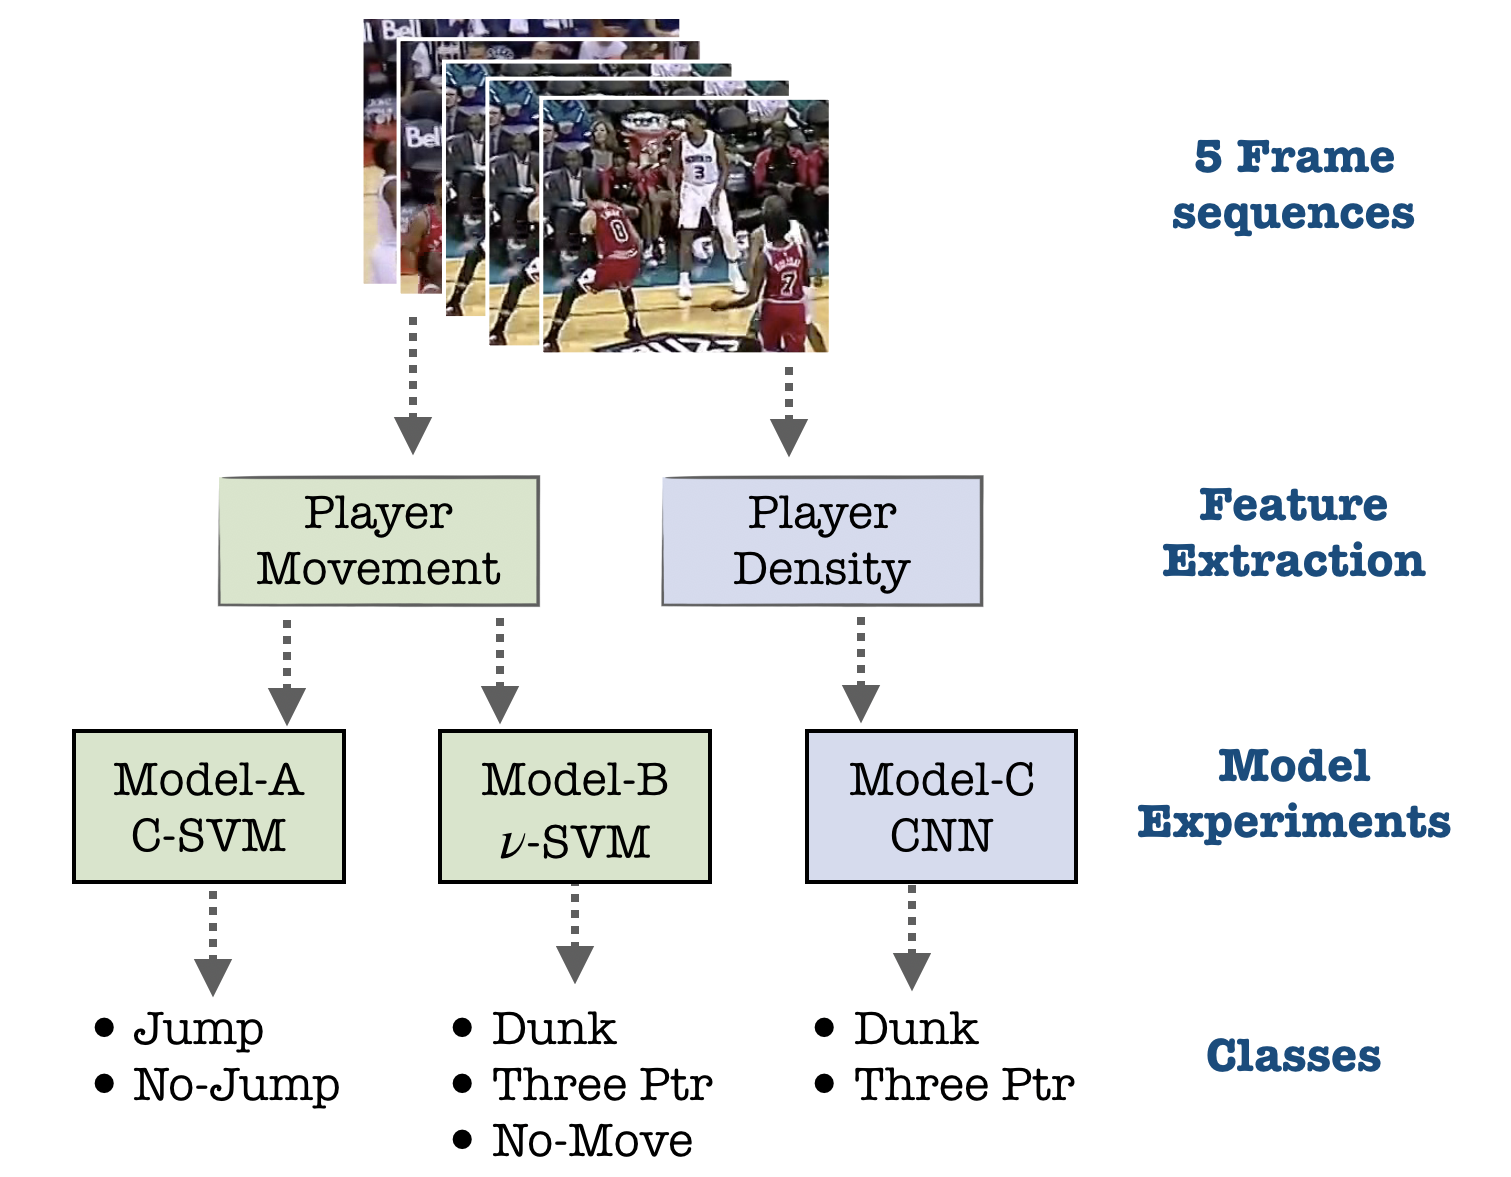
\includegraphics[width=\columnwidth]{IO.png}}
\caption{Final prediction cycle}
\label{fig:e2e}
\end{center}
\vskip -0.2in
\end{figure}


Our solution can then be trivially applied to any length of video by continuously feeding it sequences of 5  frames to identify moves in a game.

\section{Related Work}
\label{related_work}
Action recognition is a widely researched topic. Some of the most prominent methods for action recognition can be roughly organized into the following categories: 
\begin{itemize}
\item Hand-crafted features \cite{HengWang:2011:ARD:2191740.2192078,Jain_2013_CVPR,Sun_2018_CVPR},
\item Two stream neural networks \cite{NIPS2014_5353,Feichtenhofer_2016_CVPR, Carreira_2017_CVPR,Zhu_Y,Cai_2019_CVPR_Workshops},
\item 3D convolutional networks \cite{6165309,Tran_2018_CVPR},
\item Recurrent neural networks \cite{Baccouche:2010:ACS:1889001.1889024,Donahue_2015_CVPR},
\item Pose-based methods \cite{Yao_2011,Luvizon_2018_CVPR}.
\end{itemize}

These categories certainly overlap on many levels. The key strength of pose based methods and two stream neural networks is their ability to independently train spatial / temporal features and carry them from one domain to the other. This is important as the application of action recognition is vast and collection of training data costly. For example, there are dozens of "moves" in just NBA. Just trying to scale action recognition to all of NBA is hard, let alone scaling it to all of big 5 sports and chillingly hard to imagine scaling to all sports, let alone other non-sports activities. 

3D CNNs have demonstrated better performance in capturing spatio temporal structure in videos than 2D convolutions have in the past. But the biggest drawback of 3D convolutions is the large number of parameters. This makes it particularly unsuitable for fine grained action recognition in practice. Due to the sheer number of classes defined in the taxonomy of any fine grained task, the datasets are usually very small and makes it easy to overfit with the large number of parameters 3D convolutions utilize.

Two stream networks, first proposed in \cite{NIPS2014_5353}, have become popular recently. A spatial stream, analyzes a single video frame, such as utilizing Pose as a high level spatial feature. In parallel, a temporal stream uses multi-frame optical flow. This is done via a series of convolutions and fully-connected layers. For final classification, the streams are fused together via averaging or an appropriate linear model. Being separate streams, they can be trained independently with a higher likelihood of transferring from one domain to another.

Our approach uses pose as a foundation. In the first set of models, we use tracking to capture temporal features and study the ability to model common semantics underlying multiple moves, in a hope that multiple fine grained moves can then be modeled with minimum training data over sub-moves such as a "jump" that require more raw features and larger training sets to learn. In our second model, we let the CNN model the temporal movement of "aggregate player movement" which too is a foundational sub-aggregate-movement over which we can build final move classifier using scanty training data. 

Our primary motivation is the ability to scale classification to a large number of classes across a large number of sports, with minimum possible training data. For this reason, we try to break down action recognition into action proposal (semantic sub-moves / cues) and action classification (dunk, three pointer).

\section{Data}
\label{data}
One of the bottlenecks for progress in this area is the lack of open data sets with fine grained action tags. We combined two separate datasets to build a weakly supervised dataset to use as training data for this project.

%\begin{figure}[ht]
%\vskip 0.15in
%\begin{center}
%\centerline{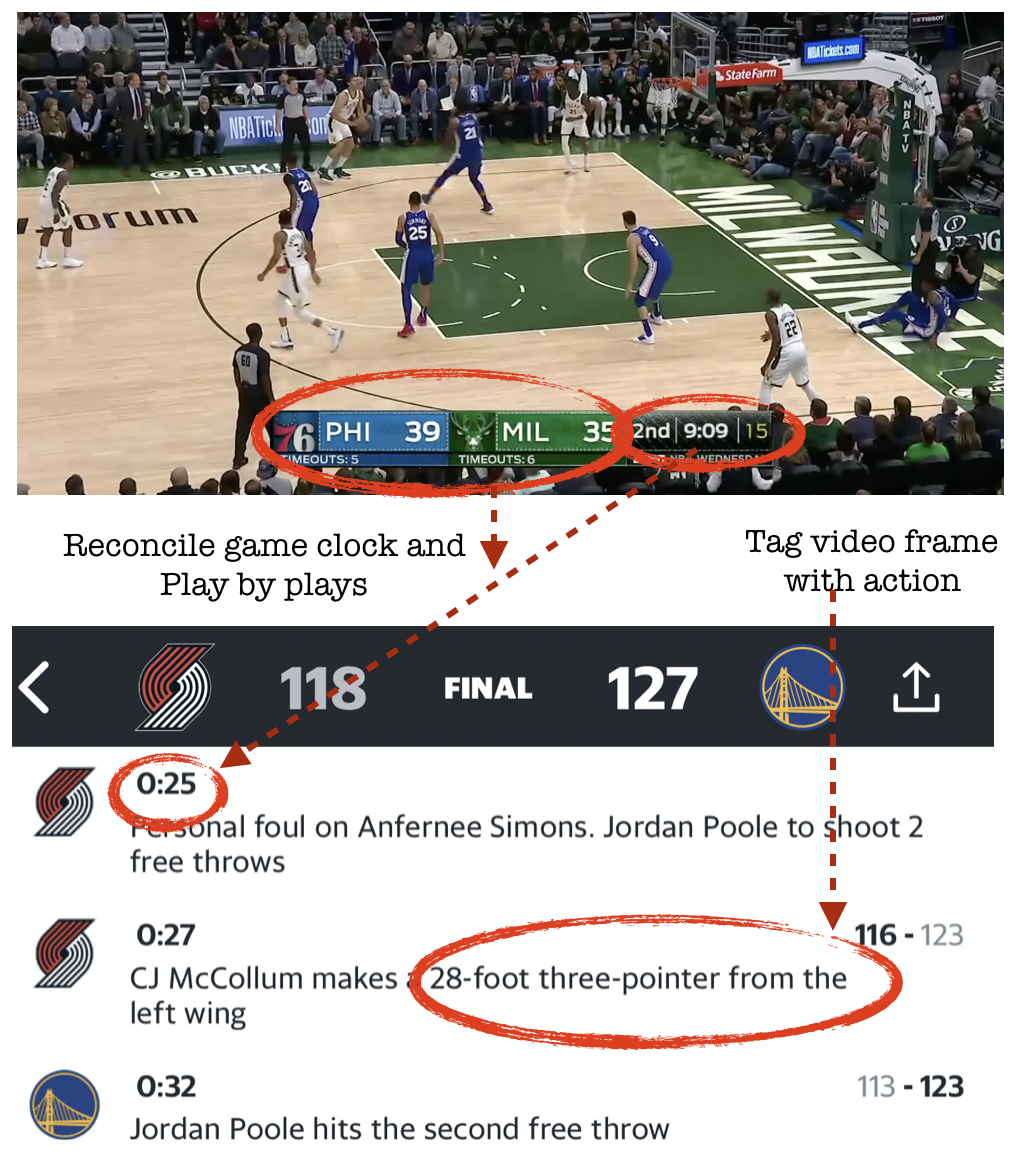
\includegraphics[width=8cm]{Data.png}}
%\caption{Data generation process}
%\label{fig:e2e}
%\end{center}
%\vskip -0.2in
%\end{figure}

\begin{figure*}[ht]
\begin{center}
\centerline{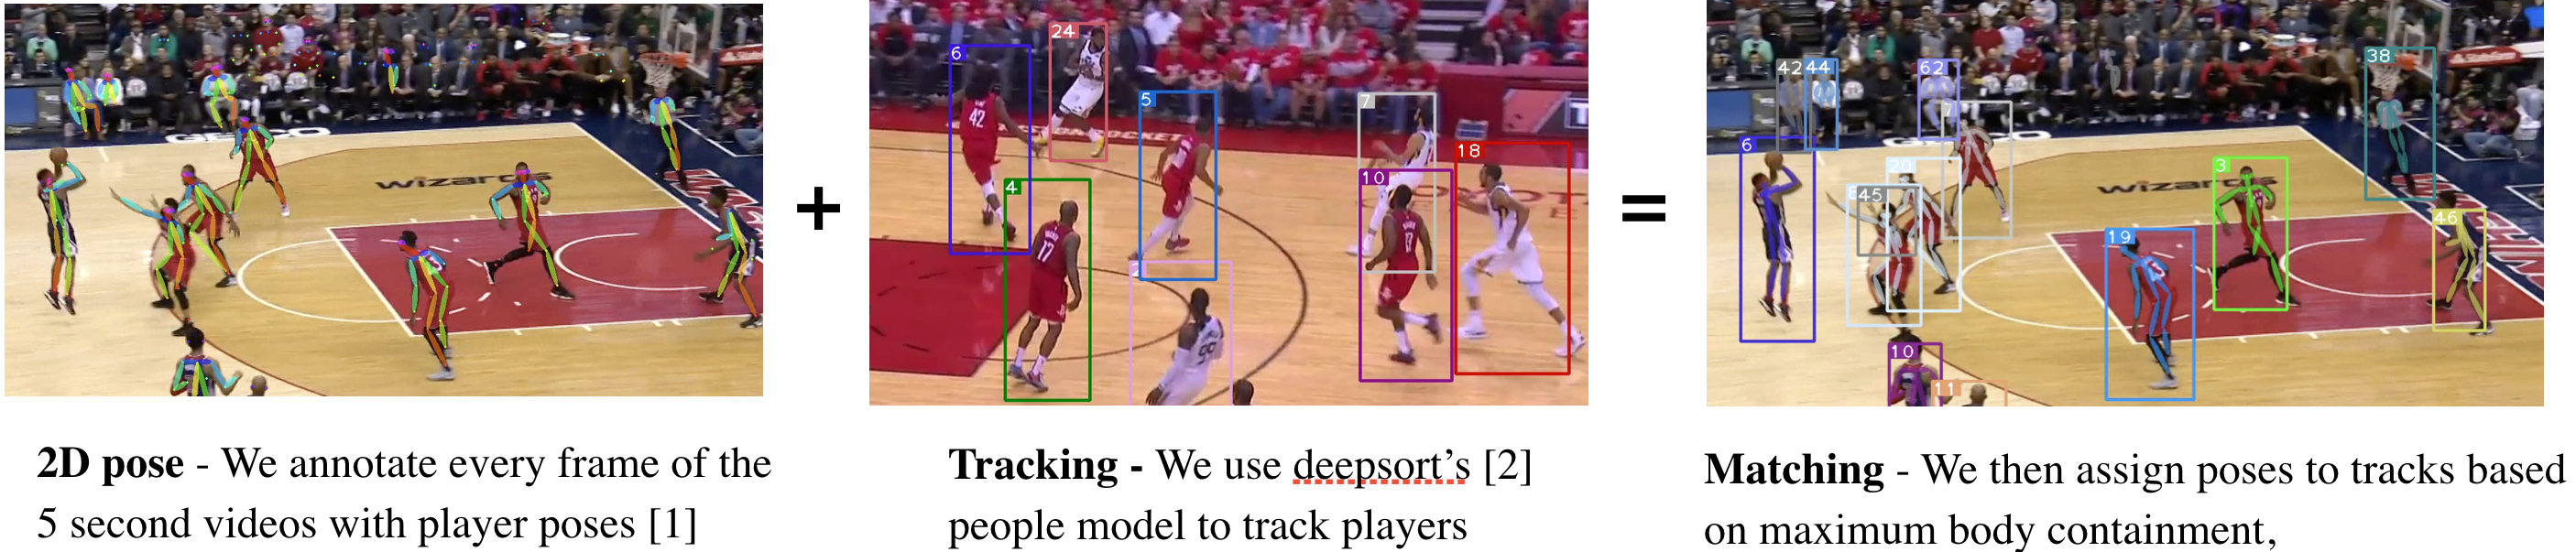
\includegraphics[height=1.5in]{trackpose.png}}
\caption{Tracked pose estimation}
\label{fig:trackpose}
\end{center}
\vskip -0.3in
\end{figure*}

Game clock in official videos from nba.com is extracted with OCR and reconciled with play by play available on sports.yahoo.com for each game. The work of fine tuning and running OCRs for video game clocks was already done and available for us to use. Structured play by plays in JSON format was also available for us to use as part of proprietary work done elsewhere.

To generate a dataset for this project, we extracted 4.5 seconds of video segments around the time play-by-plays indicated a move had occurred. After reducing the videos from 30 fps down to 10 fps, we had a data set of 240, 45-frame video segments, a frame offset where the action happened and whether the action was a dunk or a three pointer. Using simple heuristics we filtered out bad videos and tags, resulting in a total data set size of 150 video segments.

\section{Features}
\label{features}

To provide enough semantics to our final classifier we extracted temporally tracked pose features of each player in every frame of the video. This was a three step process as described in section \ref{spatiotemporal}. To address camera motion and to normalize all location and distance vectors, we also extracted approximate location of the basket in every frame. Presence of basket was also used to only predict an action on frames that contained a basket.

\subsection{Player spatio-temporal features}
\label{spatiotemporal}

Figure \ref{fig:trackpose} illustrates the three step process to create tracked poses of players. We first annotate every frame of the 5 second videos with player poses based on \cite{Cao_2017_CVPR}'s approach and open source model. We then use DeepSort \cite{Wojke2017simple} and its open source model to find bounding boxes of players that are tracked across the video. 

To assign poses to tracks we then use a simple yet effective approach of maximum pose and bounding box intersection on a frame by frame basis. We iteratively pair tracks with poses based on maximum ranked intersections, removing them from the matching process once paired. The simple approach did introduce fickleness of assignment during occlusion and crowding scenarios. But we saw only minimal effect on the recall of our final classification. Adding jersey color to provide consistency through occlusion / crowding scenarios may be an easy trick to increase the effectiveness of pairing. Though, the best approach here will be to combine both pose and tracking into a single optimization.

\subsection{Basket to fix origin}
\label{basket}

To avoid creating a basket specific bounding box, given the time constraint, we used the location of the basket holder's banner ad as a proxy for basket detection. We used Amazon's Rekognition text detection and recognition model available as an AWS service and added appropriate offsets to approximate the location of the basket in a frame. Intermittent frames that were not detected by Amazon's Rekognition were "smoothed" by fitting a straight line travel between previous and next known locations of the basket. We then transformed all player pose vectors to be relative to the new origin we fixed at the basket.

\begin{figure}[ht]
\vskip -0.05in
\begin{center}
\centerline{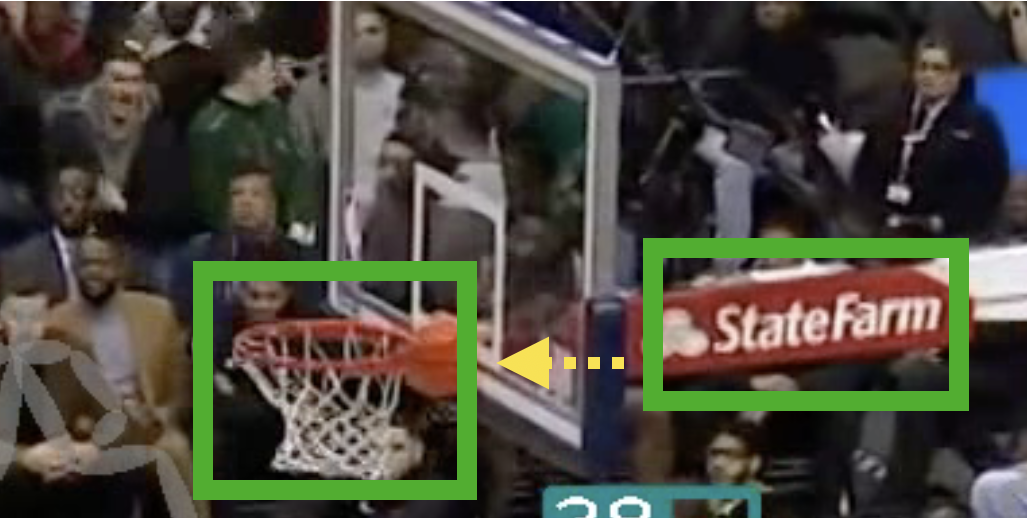
\includegraphics[width=6cm]{basket_loc.png}}
\caption{Approximating basket location}
\label{fig:basket_loc}
\end{center}
\vskip -0.2in
\end{figure}

\subsection{Aggregate features}
\label{aggregate_features}

\subsubsection{Player density}
\label{player_density}
For every frame, we calculate density of players in different regions of the court. For distinguishing between a three pointer and dunks, we only needed to group players into 'far' (yellow) and 'near' (blue) regions that mimic the shape of D around the basket. We filtered out audience by requiring them to have a minimum pose height and distance relative to the basket, without which grouping of poses was also skewed towards where the audience was.

\begin{figure}[ht]
%\vskip 0.15in
\begin{center}
\centerline{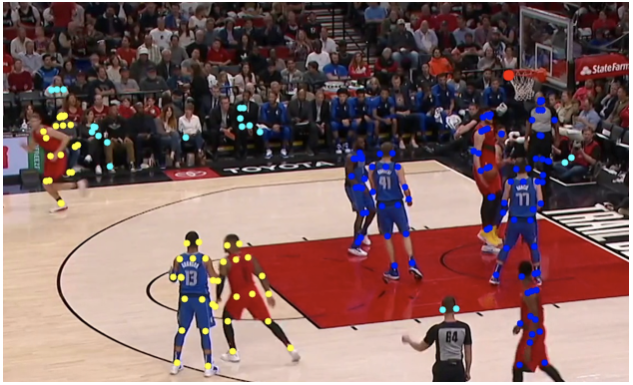
\includegraphics[width=6cm]{player_density.png}}
\caption{Player density}
\label{fig:e2e}
\end{center}
\vskip -0.2in
\end{figure}

\subsubsection{Player movement}
\label{player_movement}
For every track and every frame we also calculate the minimum and maximum change in Y coordinate, over the last 5 frames, of the pose's mean and the number of times it had its arms raised.

\section{Methods}
\label{methods}

There is always a very high number of classes defined in the taxonomy of any fine grained task. As a result, datasets available for such tasks are also small. To validate the hypothesis that we can learn to classify fine grained actions over a common set of separately learnt sub-actions or action proposal events, we model three SVMs that work with aggregate player movement and one CNN model that tracks changes in player densities. 

\subsection{Classification based on Pose movement}
Our first method for classification is based on the activity of each individual player via its pose features across the previous 5 frames.

Learning algorithms such as Support Vector Machines (SVM) accept fixed size vectors and cannot work with varying sizes. Number of players and their body parts that we are able to identify varied from one frame to another. In order to benefit from various learning techniques, we needed a mechanism to aggregate sets of local features into discriminative and fixed-size descriptors. So, we pre-aggregated player movement features as described in section \ref{player_movement}.

We define the following aggregate and raw feature names:
\begin{itemize}
\item X,Y = mean distance of pose from basket
\item dY = change in Y w.r.t. last 5 frames of a track
\item A = number of times pose’s arms were up over the last 5 frames
\end{itemize}

\subsubsection{C-SVM: Action Proposal}
Here we learn to classify a sequence of 5 frames as containing or not containing a jump by any player on the court. To handle class imbalance between hard-to-find jumps and always-there no-jumps, we use C-SVM so we can separately tune mis-classification costs for jumps vs no-jumps.

\begin{figure}[ht]
\vskip -0.05in
\begin{center}
\centerline{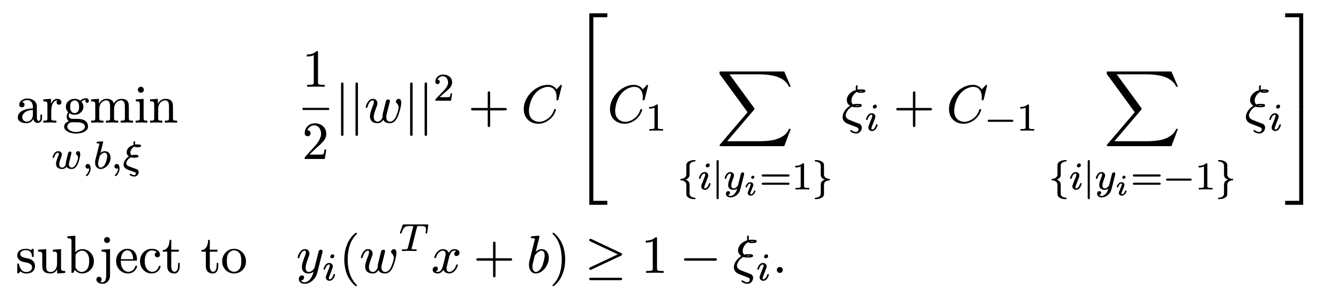
\includegraphics[width=\columnwidth]{csvm_equation.png}}
\label{fig:csvm_equation}
\end{center}
\vskip -0.2in
\end{figure}

This classifier is run on every track identified in every frame of a given video, to identify the frame and x,y coordinate of a jump, if any. Input features to this algorithm is a 3 element vector per frame, $F=[min(dY), max(dY), A]$

\subsubsection{$\nu$-SVM: Action Recognition over Proposal}
For the frames that we know a jump occurred, we then write a classifier to demonstrate how most fine grained classification can be trivially built over common sub moves / events / action proposals. 
\begin{figure}[ht]
\vskip -0.05in
\begin{center}
\centerline{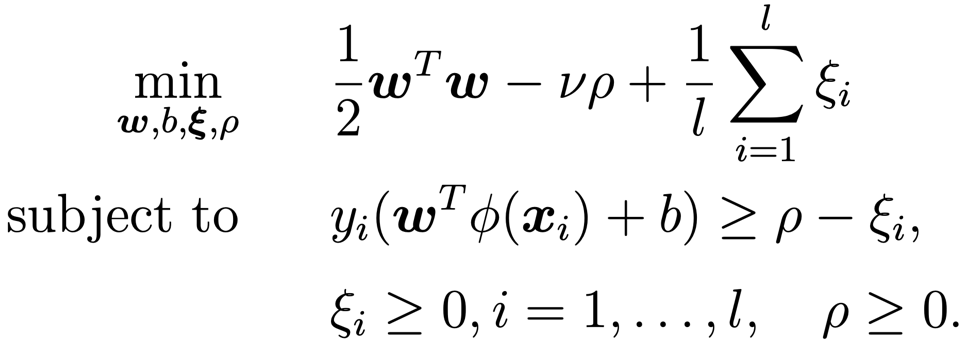
\includegraphics[width=6cm]{nusvm_equation.png}}
\label{fig:nusvm_equation}
\end{center}
\vskip -0.2in
\end{figure}
Here we use a simple $\nu$-SVM with a feature vector [X, Y] representing the jump location.

\subsubsection{$\nu$-SVM: Single step Action Recognition}
To demonstrate that joint models can be easily built once underlying semantic components have been identified, we simply concatenate the feature set of previous two models as $F=[min(dY), max(dY), A, X, Y]$ to train a one step fine grained classification model, again using $\nu$-SVM.

\subsection{Classification based on player density shifts}
To model another semantic sub component, we model the fine grained classification by training a CNN to learn how player density patterns shift differently across frames between a dunk and a three pointer. Due to scanty training data we feed the CNN pre-aggregated notion of player densities and only train the CNN to learn the shift pattern as shown below:

\begin{figure}[ht]
\vskip -0.05in
\begin{center}
\centerline{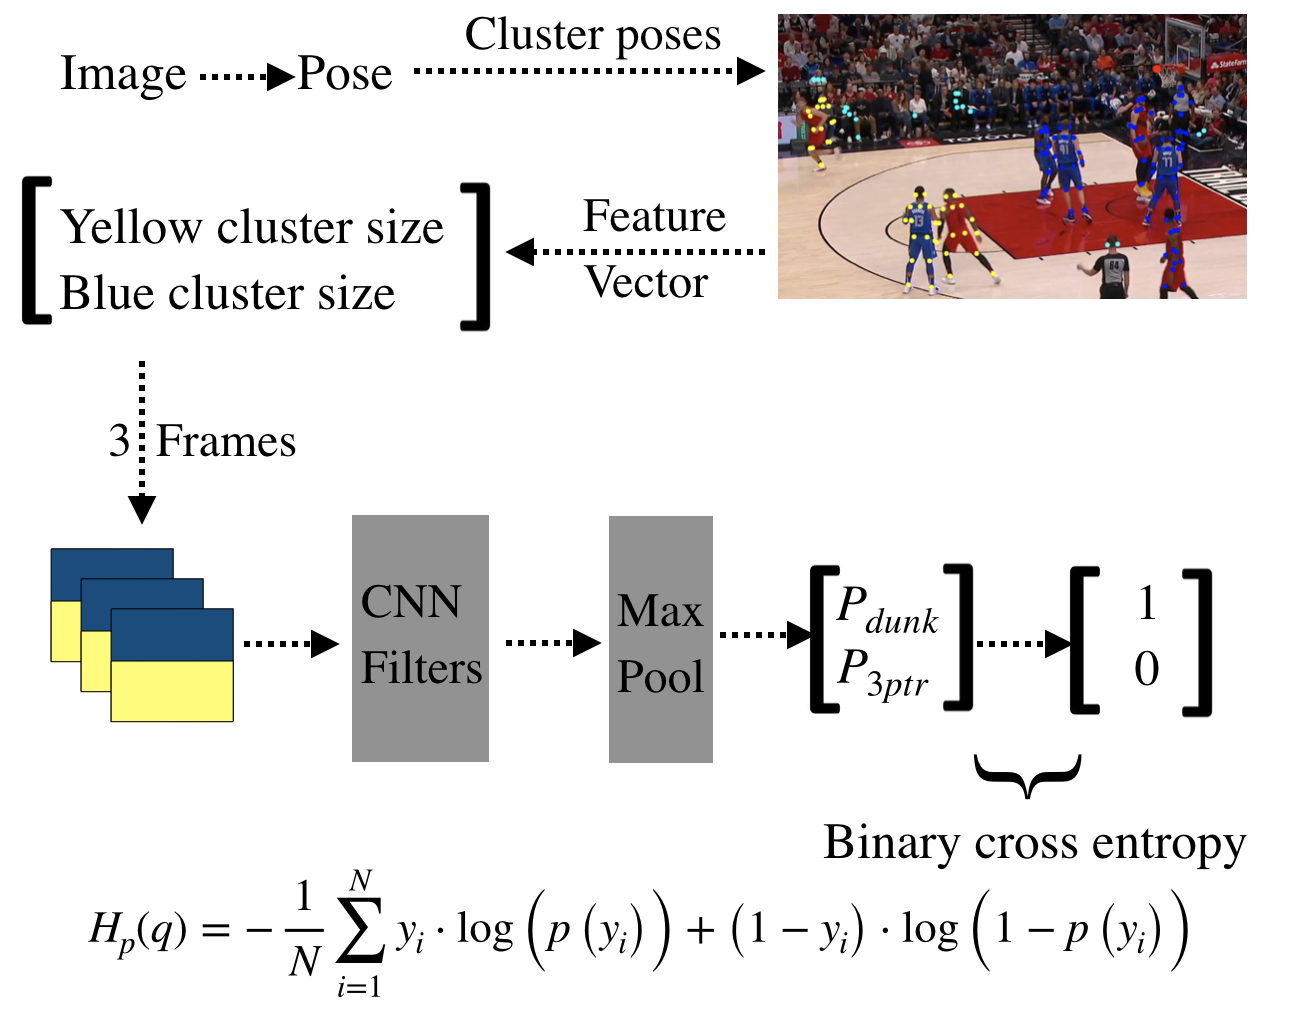
\includegraphics[width=\columnwidth]{cnn.png}}
\label{fig:e2e}
\end{center}
\vskip -0.2in
\end{figure}

We use binary cross entropy to train our probabilities against one class label setting. We run CNN filters of size 1 and size 2 over the input matrix $\in \mathbb{R}^{3 \times 2}$ to capture relative densities within a frame and across frames sequences.

\section{Experiments, Results and Discussion}
\label{methods}
We trained the first C-SVM model that predicts Jump vs No-Jump with 89 positive and 306 negative examples of jumps. Positives were capped by how many videos we were able to manually label. For negatives we programmatically picked frame sequences that would be a close match to a jump, for example, when players had their arms raised, or their mean Y suddenly increased over consecutive frames. We wanted to capture some variations in poses that looked like jumps, but weren't. We did a 80/20 train/test split. During our first try, the model learnt to almost always classify everything as not a Jump. To handle the class imbalance, we set mis-classification weight for Jumps to 22 and no-jumps to 1. Were were able to achieve accuracies of 76.71\% and 85.55\% on training and test sets.

To demonstrate building simple classifiers over common semantic events, we trained a trivial model that classified a jump event to be a dunk vs three pointer based on location of of a jump event (action proposal). We unsurprisingly achieved accuracies of 96 and 98\% on train and test sets.

Finally, we trained a joint $\nu$-SVM model as a multi-class classifier (Dunk, Three pointer, No-Move) over a concatenated feature set of the previous two classifiers. We set $\nu = 0.155$. We arrived at the optimum $\nu$ by starting at 0.5 and following the direction of max performance in a gradient descent like manner.

We designed the CNN to learn patterns of change in player density across the court. After filtering out audience, we were able to achieve good accuracies around 1000 epochs. Please see Figure \ref{fig:cnn_train_loss} for progression of  training. We used 4 set of size 1 and size 2 filters, standard adam gradient descent and sigmoid activation for the dense layer. 

%We took an objective to break down moves into their semantic components, such as run, jump, dribble etc. And it works as we show it with SVMs. So, we don’t need lots of training data for each individual move from the broadcast videos and can stitch moves with more generically learnable sub-moves.


%We have boiled it down to semantics and then applied cnn. But it is our goal to do on the raw features of pose and tracks. We wanted to verify the semantics. v imp to see the different semantics coming out. We see, but in some cases we don’t see it coming out. As training progress we want to verify the semantics are coming out. Thresholded features will become metrics or addiotnal semantic pieces in the loss function. Semantics constraints coming in as regularization terms in the loss function. 

\begin{table}[t]
\label{sample-table}
\vskip 0.15in
\begin{center}
\begin{small}
\begin{sc}
\begin{tabular}{lcccr}
\toprule
Model & Train & Test \\
\midrule
Pose movement models \\
\midrule
C-SVM Proposal Only   & 76.71\% & 85.55\% \\
$\nu$-SVM Recognition & 96.0\% & 98.22\% \\
$\nu$-SVM Joint Model    & 87.59\% & 85.56\% \\
\midrule
Player density model \\
\midrule
CNN     & 92.21\% & 98.43\% \\
\bottomrule
\end{tabular}
\end{sc}
\end{small}
\end{center}
\caption{Classification accuracies.}
\vskip -0.1in
\end{table}

\begin{figure}[ht]
\vskip 0.15in
\begin{center}
\centerline{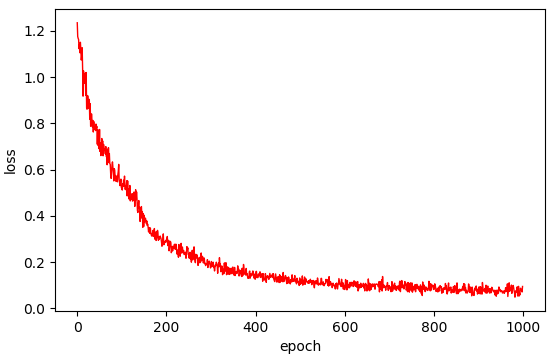
\includegraphics[width=\columnwidth]{cnn_train_loss_font.png}}
\caption{CNN training loss}
\label{fig:cnn_train_loss}
\end{center}
\vskip -0.2in
\end{figure}

\begin{figure}[ht]
\vskip 0.05in
\begin{center}
\centerline{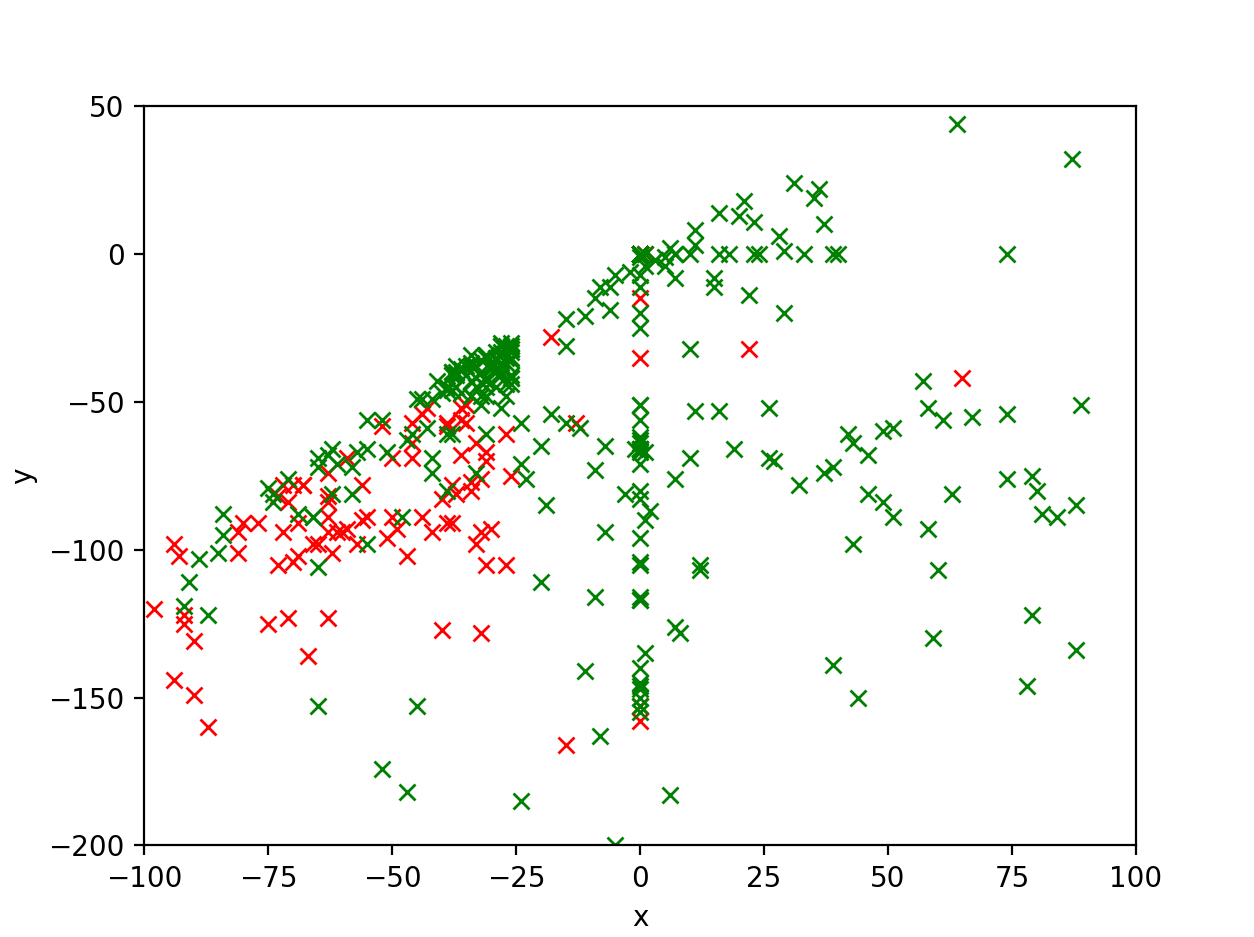
\includegraphics[width=\columnwidth]{xy_travel.png}}
\caption{Player movement dY and dX features}
\label{fig:classes}
\end{center}
\vskip -0.3in
\end{figure}

The two most difficult issues we faced were:
\begin{itemize}
\item Pose estimation and tracking in key frames - Key action frames are often occluded. Player poses are often missing key joints and limbs right when they are most needed. Right when the player hangs on the basket or jumps to make a dunk or three pointer. A joint model for pose and tracking with regularization to encode semantics / constraints of a particular sport will greatly help here. This aspect had the biggest impact on the quality of predictions.
\item Noise from audience - Noise filtering was not a problem at with the SVMs as they were trained on individual player movement. Audience don't move. Where-as we had to aggressively filter out audience to get reasonable performance out of our CNNs. We need more algorithmic ways of filtering out audiences.
\end{itemize}


%We don’t need too much of training data for these dunks and kind of works with small example . Because semantics has worked out. 

\section{Conclusion and Future Work}
\label{conclusion}
Fine grained action recognition is an important area of research. It can be overwhelming, but we think, if we break it down into a set of semantics such as "jump", "dribble", "group movement" that are few and are possible to learn from large data sets outside of each specific domain, it is possible to train fine grained action recognition with minimal training data which is key to scaling any practical application across a large taxonomy of fine grained actions across a long list of sports. 

The next step would be to build a joint model between pose estimation and tracking that can handle occlusion and crowding better. But more importantly formalize a way to model some core semantics specific to NBA or any given sports as regularization in the joint model to leverage known constraints for prediction performance when it is needed the most. We would like to source more training data and implement ways to work with weakly supervised data in a more robust way. 

\section{Code}
\label{code}
https://github.com/amitnagpal229/cs229project 

% In the unusual situation where you want a paper to appear in the
% references without citing it in the main text, use \nocite
\nocite{langley00}

\bibliography{example_paper}
\bibliographystyle{icml2019}


\end{document}


% This document was modified from the file originally made available by
% Pat Langley and Andrea Danyluk for ICML-2K. This version was created
% by Iain Murray in 2018, and modified by Alexandre Bouchard in
% 2019. Previous contributors include Dan Roy, Lise Getoor and Tobias
% Scheffer, which was slightly modified from the 2010 version by
% Thorsten Joachims & Johannes Fuernkranz, slightly modified from the
% 2009 version by Kiri Wagstaff and Sam Roweis's 2008 version, which is
% slightly modified from Prasad Tadepalli's 2007 version which is a
% lightly changed version of the previous year's version by Andrew
% Moore, which was in turn edited from those of Kristian Kersting and
% Codrina Lauth. Alex Smola contributed to the algorithmic style files.
